\section{Prilagodba za implementaciju na mikrokontroleru}
\label{sec:convert}

Veličina pojedinog sloja treniranog modela neuronske mreže prikazana je na slici \ref{pic:size}.
Ukupni broj parametara koje mreža ima iznosi 9439 što u memoriji zauzima malo manje od 
37 KB.

\begin{figure}[htb]
    \centering
    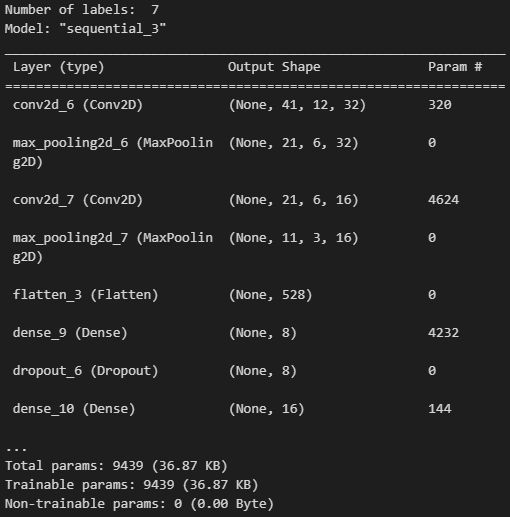
\includegraphics[width=0.65\linewidth]{Chapters/neuronska_mreza/convert/struktura.png} 
    \caption{Veličina trenirane neuronske mreže}
    \label{pic:size}
\end{figure}

Međutim, spremljeni model u memoriji osim vrijednosti parametara mora imqti i informaciju 
o samoj strukturi mreže što znatno povećava sami memorijski otisak. Datoteka s nastavkom
".pb" (engl. protobuff) čuva sve informacije potrebne za korištenje treniranog modela,
a konretni model u tom obliku zauzima nešto više od 173 KB. Korištenje takvog modela
na mikrokontroleru nije prihvatljivo niti zbog veličine niti zbog oblika zapisa. Zbog 
toga je potrebno prilagoditi model. Tensorflow Lite biblioteka omogućava vrlo jednostavnu
promjenu formata spremanja informacije o treniranom modelu. Format s nastavkom ".tflite"
sažima model na nešto više od 41 KB. Međutim, postoji još nešto što je moguće napraviti
kako bismo saželi model još više te ga pretvorili u oblik pogodan za korištenje na
mikrokontroleru. Spomenuta metoda sažimanja zove se kvantizacija, a oblik u kojem će model
biti spremljen zove se "flatbuffer".

Kvantizacija je metoda optimizacije modela kojom se smanjuje broj bitova potrevnih za
spremanje informacije o parametrima modela. Ova redukcija preciznosti (s 32 na 8 bitova)
pridonosi smanjenju veličine modela i ubrzanju izvođenja, a neznatno utječe na točnost
modela \cite{}. Ovim zahvatom veličina modela smanjena je na 16 KB. 

Flatbuffer je oblik za serijalizaciju podataka razvijen u Googleu. Dizajniran je
za učinkovitu pohranu i pristup podacima \cite{}. 
Pretvorbom treniranog modela u ovakav oblik
dobiveno je polje podataka spremno za korištenje programskim jezikom C.

Tablica \ref{tab:model_sizes} prikazuje veličine modela u različitim koracima prilagodbe.
Konačni model prihavtljive je veličine za implementaciju na mikrokontrolerskom sustavu, 
a iznosi svega 9\% početne veličine modela.

\begin{table}[htb]
    \centering
    \begin{tabular}{|l|r|}
        \hline
        \textbf{Model} & \textbf{Veličina(B)} \\ \hline
        Početni model & 173241\\ \hline
        TF Lite & 41644 \\ \hline
        TF Lite + kvantizacija & 15704 \\ \hline
    \end{tabular}
    \caption{Veličine različitih oblika modela}
    \label{tab:model_sizes}
\end{table}